% Basics of discretizations and solvers

\section {Discretizations and numerical solvers}

\begin {frame} [t]
\frametitle {Numerical solution of the PDE}
\vspace {-2ex}
The classical approach includes the following phases:
\begin {enumerate}
	\item {\color{blue}Discretization}: The continuum domain $\Omega$ is replaced by a {\color{blue} grid}
		$\Omega_h$, $u$ by $u_h$ from a finite-dimensional space, the differential
		operator by an algebraic operator between finite-dimensional spaces. Therefore, the
		PDE is converted to a {\color{blue}large sparse system of algebraic equations}. \\
	\pause
	\item Solution of the algebraic system. The {\color{blue} solver} should be enough efficient for the
		system of this size. It should profit from the sparsity, hardware architecture etc. \\
		Keywords: Newton's method, CG, BiCGStab etc. iterations, GMG, AMG preconditioners,
		ILU, GS smoothers etc.
\end {enumerate}
\end {frame}

\begin {frame} [t]
\frametitle {Diffusion equation (stationary case)}
$$
 \begin{array} {rcll}
  - \nabla \cdot (d \nabla u) & = & f, & x \in \Omega \subset \mathbb{R}^2 \\
  u & = & g_D, & x \in \Gamma_D \\
  \mathbf{D} \nabla u \cdot \mathbf{n} & = & 0, & x \in \Gamma_N 
 \end{array}
$$
where
\begin {itemize}
	\item $\mathbf{D} = \mathbf{D} (x) \in \mathbb{R}^2$ is the diffusion tensor,
	\item $f = f (x) \in \mathbb{R}$ are the sources,
	\item $\Gamma_D \cup \Gamma_N = \partial \Omega$, $\Gamma_D \cap \Gamma_N = \emptyset$
		are Dirichlet and Neumann boundaries
	\item $g_D = g_D (x) \in \mathbb{R}$ are the Dirichlet values,
	\item $\mathbf{n}$ is the outer normal.
\end {itemize}
\end {frame}

\begin {frame} [t]
\frametitle {Shape functions}
Discrete solution $u_h$ is represented as
$$
 u_h (x) = \sum_{i = 1}^{N} u_i \lambda_i (x),
$$
where $\lambda_i: \Omega \to \mathbb{R}$ are continuous piecewise (multi-) linear with
\centerline {$\lambda_i (x_i) = 1, \quad \lambda_i (x_j) = 0 \quad (j \ne i)$ (``hat functions'').}

\pause
\vspace {2ex}
\centerline {$u_i$: ``{\color{blue} degrees of freedom}'' (assigned to the {\color{blue} vertices})}

\pause
\vspace {2ex}
In ug4, DoFs can be assigned locally to any part of any type of grid elements. This assignment
and the local interpolation rule is refered to as ``{\color{blue} ApproximationSpace}''.
In the present example, it is ``{\color{blue} Lagrange, order 1}''. On every grid level,
the assignment is managed using its ``{\color{blue} DoFDistribution}''.
\end {frame}

\begin {frame} [t]
\frametitle{Finite Volumes: Dual grid}
\centerline{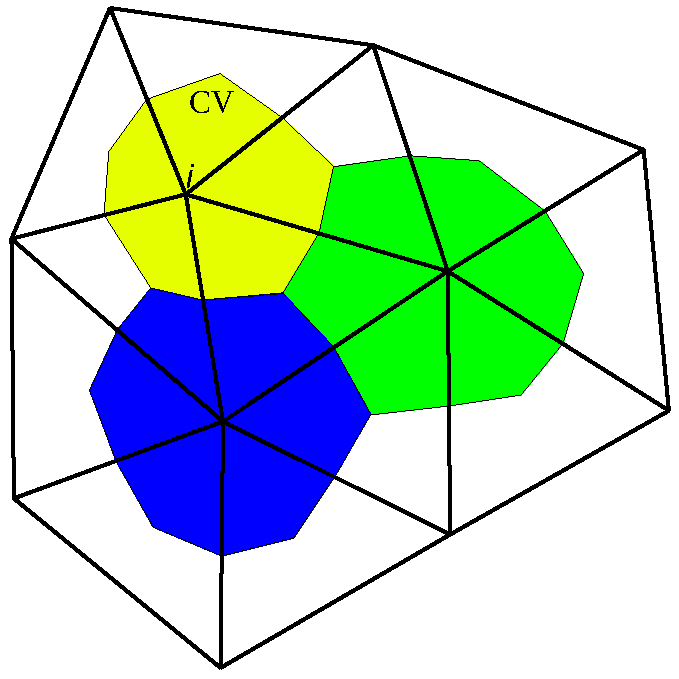
\includegraphics [width=0.6\textwidth] {FV-Elem-Donald-Scheme.pdf}}
\only<1>
{%
\centerline{Donald Diagrams: Connect the midpoints.}
}%
\only<2>
{%
\centerline {$\displaystyle - \nabla \cdot (\mathbf{D} \nabla u) = f$}
}%
\only<3>
{%
\centerline {$\displaystyle - \int_{\mathrm{CV}} \nabla \cdot (\mathbf{D} \nabla u) \, dx = \int_{\mathrm{CV}} f \, dx$}
}%
\only<4>
{%
\centerline {$\displaystyle - \int_{\mathrm{\partial CV}} (\mathbf{D} \nabla u) \cdot \mathbf{n} \, dx = \int_{\mathrm{CV}} f \, dx$}
}%
\end {frame}

\begin {frame} [t]
\frametitle{Finite Volume Finite Element Method}
\centerline{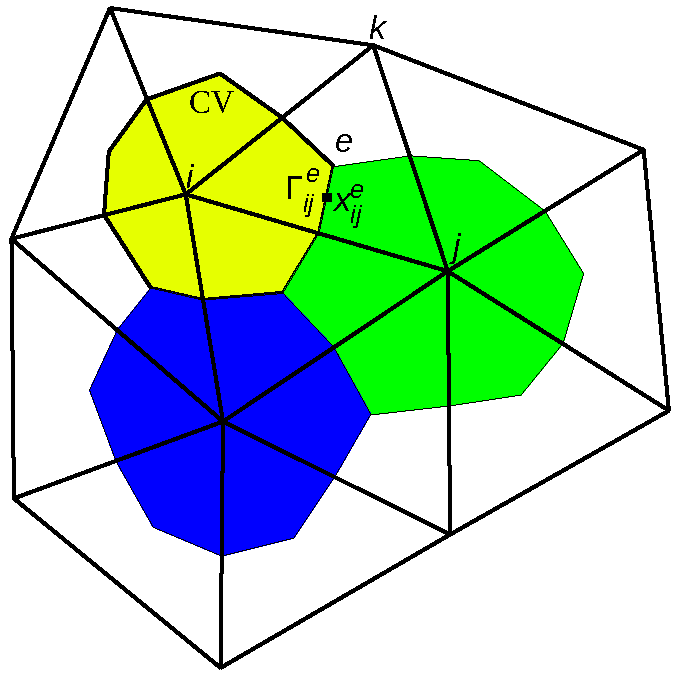
\includegraphics [width=0.6\textwidth] {FV-Elem-Donald.pdf}}
\only<1>
{%
\centerline{$\Gamma^{e}_{ij}$: ``{\color{blue} subcontrol volume face}'', $x^{e}_{ij}$: its ``{\color{blue} integration point}''}
}%
\only<2>
{%
\centerline{$\displaystyle \nabla^e u_h = \sum_i u_i \nabla^e \lambda_i$: a linear combination}
}%
\only<3>
{%
\centerline{$\displaystyle - \sum_{e \ni x_i} \sum_{j \ne i} | \Gamma^e_{ij} | \mathbf{D}^e_{ij} \nabla^e u_h \cdot \mathbf{n}^e_{ij} = | \mathrm{CV}_i | f_i$}
}%
\end {frame}

\begin{frame} [t]
\frametitle {Neumann Boundary Conditions}
\centerline{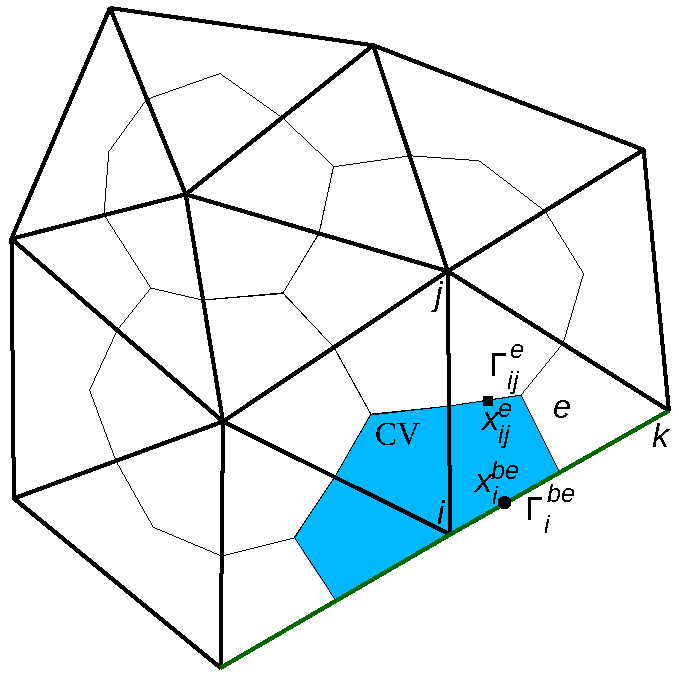
\includegraphics [width=0.6\textwidth] {FV-Elem-Donald-bnd.pdf}}
\centerline{%
$
 \left .  \mathbf{D} \nabla u \cdot \mathbf{n} \right |_{\Gamma_N} = g_N: \,
 \displaystyle
 - \sum_{e \ni x_i}
  \bigl (
   \sum_{j \ne i} | \Gamma^e_{ij} | d^e_{ij} \nabla^e u_h \cdot \mathbf{n}^e_{ij}
   +
   | \Gamma^{be}_{i} | g_{N,i}
  \bigr )
 = | \mathrm{CV}_i | f_i
$%
}
\end{frame}

\begin{frame} [t]
\frametitle {Non-linear equations}
Discretized non-linear algebraic system of algebraic equations on $\Omega_h$:
$$
 \mathcal{A} (u) = 0
$$
\begin{itemize}
 \pause
 \item ``Sparse'': Every equation depends only on a small number of DoFs for any $h$.
 \pause
 \item It may have several solutions $u$. However, typically it is assumed that $u$ is unique.
 \pause
 \item $\mathcal{A}$ should be differentiable at least in a neighbourhood of the solution.
\end{itemize}
\end{frame}

\begin{frame} [t]
\frametitle {Iterative non-linear solvers}
\dots compute a sequence
$$
 u_0, u_1, u_2, \dots, u_k, \dots
$$
that should converge to the solution $u_{*}$ of $\mathcal{A} (u) = 0$.

\pause
\vspace{2ex}
$d_k := \mathcal{A} (u_k)$ is said to be the \emph{defect} of $u_k$.

\pause
\vspace{2ex}
The system is linearized. We denote by $\mathbf{A}_k$ the Jacobian of
$\mathcal{A}$ at $u_k$. By $\tilde{\mathbf{A}}_k$, we denote its approximation, e.g.
$\tilde{\mathbf{A}}_k = \mathbf{A}_k$.

\pause
\vspace{2ex}
Typical iteration:
$$
 u_{k+1} = u_k - \alpha_k \tilde{\mathbf{A}}_k^{-1} \mathcal{A} (u_k)
$$
with \emph{step length} $\alpha_k$ (obtained by linesearch).
\end{frame}

\begin{frame} [t]
\frametitle {Implementation of the non-linear solvers}
\begin{itemize}
 \item The non-linear operator $\mathcal{A}$ cannot be represented in the memory
  (in contrast to the sparse matrix $\tilde{\mathbf{A}}_k$).
 \pause
 \item Instead, one implements functions evaluating \emph{grid function} $d_k = \mathcal{A} (u_k)$
  and the large sparse matrix $\tilde{\mathbf{A}}_k$ for every $u_k$.
 \pause
 \item To get $\tilde{\mathbf{A}}_k^{-1} \mathcal{A} (u_k)$, solve the system
  $$
   \tilde{\mathbf{A}}_k c_k = d_k
  $$
  (e.g. by the GMG method).
 \pause
 \item The discretization modules in ug4 implement computation of $\tilde{\mathbf{A}}_k$
  and $d_k$ for any $u_k$. (This is denoted by ``{\color{blue} \emph{assembling}}''.) 
 \pause
 \item Analogously in the non-stationary case.
\end{itemize}
\end{frame}

% End of File
